\documentclass{scrartcl}
\usepackage{amsmath}
\usepackage{riley}
\usepackage{riley-libertine}
\usepackage{xfrac}

\usepackage{multicol}
\usepackage{tikz}

\begin{document}
\section{Polar coordinate}
\[
  ds^2 = dr^2 + r^2 d\theta^2
\]
Lagrangian
\[
  L = \frac{\dot r^2}2 + r^2 \frac{\dot\theta^2}2
\]
\[
  \frac{\partial L}{\partial \dot r} = \dot r \quad \frac{\partial L}{\partial \dot\theta} = r^2 \dot \theta \implies L = H
\]
Momentum conservation:
\[
  r^2\dot \theta = B \implies \dot\theta = B / r^2
\]
Energy conservation:
\[
  2E=A^2 = \dot r^2 + r^2 \dot \theta^2 = \dot r^2 + r^2 \paren{B/r^2}^2  = \dot r^2 + B^2/r^2
\]
\[
  dr = dt \sqrt{A^2 - B^2/r^2}
\]
\[
  dt = \frac{dr}{\sqrt{A^2 - B^2/r^2}} = \frac{r\,dr}{\sqrt{A^2r^2 - B^2}}
\]
\(r = \paren{\sfrac{B}{A}}\cosh u\) and \(dr = \paren{\sfrac{B}{A}} \sinh u\,du \)
\[
t = \int \frac{\sfrac{B^2}{A^2}\cosh u \sinh u\, du}{B\sinh u} = \frac{B}{A^2} \sinh u = \frac{B}{A^2}\sqrt{\sfrac{A^2}{B^2}r^2 - 1 } = \frac{\sqrt{A^2r^2-B^2}}{A^2}
\]
\[
  \paren{A^2t}^2 = A^2 r^2 -B^2 \implies r^2 = \frac{\paren{A^2 t}^2 + B^2}{A^2} = A^2t^2 + \paren{\sfrac{B}{A}}^2
\]
\[
  r= \sqrt{A^2t^2 + \paren{\sfrac{B}{A}}^2} = \sqrt{A^2t^2 + {r_0}^2}
\]
\[
  d\theta = \frac{A\,dt}{A^2t^2+{r_0}^2} \quad t = \sfrac{r_0}A \tan u \quad dt = \sfrac{r_0}{A} \sec^2 u \,du
\]
\[
  \Delta\theta =  \int \frac{A \sfrac{r_0}A \sec^2u\,du }{\sqrt{{r_0}^2}\sec^2 u} = u = \tan^{-1}\paren{\frac{At}{r_0}}
\]
\section{sphere}
\[
  ds^2 = d\rho^2 + \sin^2\rho\, d\theta^2
\]
\[
  L = \frac{\dot \rho^2}{2} + \sin^2\rho \frac{\dot \theta^2}{2}
\]
Momentum:
\[
  {\sin^2\rho}\,\dot\theta = B \implies \dot\theta = \frac{B}{\sin^2\rho}
\]
Energy conservation:
\[
  A^2 = 2E = {\dot \rho^2} + {\sin^2\rho}\, {\dot \theta^2} = \dot\rho^2+ \frac{B^2}{\sin^2\rho}
\]
\[
  dt = \frac{d\rho}{\sqrt{A^2-{B^2}/{\sin^2\rho}}} = \frac{\sin\rho\, d\rho}{\sqrt{A^2\sin^2\rho - B^2}}
\]
\[
  d\theta = \frac{B}{\sin^2\rho} dt = \frac{B\, d\rho}{\sin\rho \sqrt{A^2\sin^2\rho-B^2}}
\]
\section{light cone coordinates}
\begin{multicols*}{2}
  \begin{align*}
    C &= \frac1{\sqrt 2}
        \begin{bmatrix}
          1 & 1 \\ 1 & -1
        \end{bmatrix} \\
    C^2&= \frac12
         \begin{bmatrix}
           2 \\ & 2
         \end{bmatrix} = I
  \end{align*}
  so it's idempotent.

  Metric
  \begin{align*}
    \eta(x,y) &= \eta_{s} \paren{C^{-1}x,C^{-1}y} \\
              &= \eta_{s} \paren{Cx,Cy} \\
              &= x^TC^T\eta_s C y \\
    C\eta_s C &= \frac1{ 2 }
                  \begin{bmatrix}
                    1 & 1 \\
                    1 &-1
                  \end{bmatrix}
                  \grayunderbrace{
                  \begin{bmatrix}
                    1 \\ & -1
                  \end{bmatrix}
                  \begin{bmatrix}
                    1 & 1 \\
                    1 &-1
                  \end{bmatrix}}{
                  \begin{bmatrix}
                    1 & 1 \\ -1 & 1
                  \end{bmatrix}
                  }
                  \\
    \eta&=
      \begin{bmatrix}
        & 1 \\ 1
      \end{bmatrix} \\
    \begin{bmatrix}
      a \\ b
    \end{bmatrix}
    \cdot
    \begin{bmatrix}
      c \\ d
    \end{bmatrix}
    &=
      \begin{bmatrix}
        a & b
      \end{bmatrix}
      \begin{bmatrix}
        &1\\ 1
      \end{bmatrix}
      \begin{bmatrix}
        c \\ d
      \end{bmatrix} \\
    &=ad + bc
    \\
    \abs{
    \begin{bmatrix}
      x \\ y
    \end{bmatrix}
    }_\eta^2  &=2xy
  \end{align*}
  Boosts
  \begin{align*}
    CBC^{-1} &=
          \frac12
          \begin{bmatrix}
            1 & 1 \\ 1 & -1
          \end{bmatrix}
          \grayunderbrace{
          \begin{bmatrix}
            c & s \\
            s & c
          \end{bmatrix}
          \begin{bmatrix}
            1 & 1 \\
            1 & -1
          \end{bmatrix}
          }{
          \begin{bmatrix}
            c+s & c- s \\
            c+s & s-c
          \end{bmatrix}
          } \\
    &=
      \begin{bmatrix}
        c+s & 0 \\
        0 & c-s
      \end{bmatrix} \\
    &=
      \begin{bmatrix}
        e^t \\ & e^{-t}
      \end{bmatrix}
  \end{align*}
  \[
    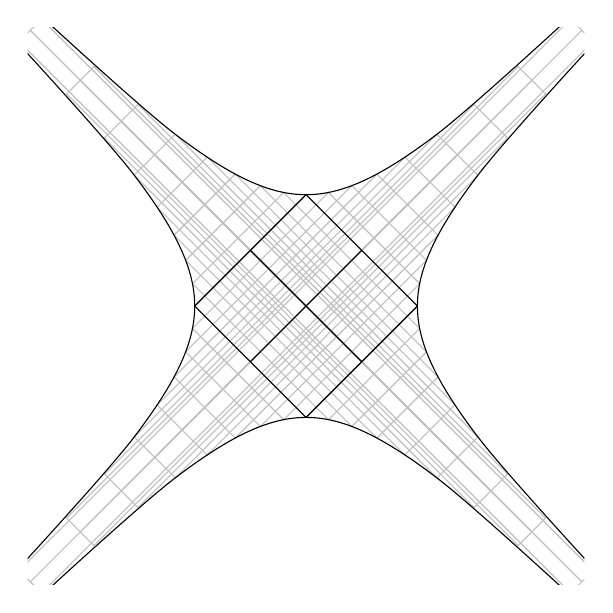
\begin{tikzpicture}[rotate=45]
      \def\L{5}
      \clip (-\L,0)   -- (0,\L) -- (\L,0) -- (0,-\L) --cycle;
      \foreach \t in {0,0.2,...,1.6}
      \draw[lightgray]
      (0,0) rectangle ({exp \t},{exp -\t})
      (0,0) rectangle ({exp -\t},{exp \t})
      (0,0) rectangle ({exp \t},{-exp -\t})
      (0,0) rectangle ({exp -\t},{-exp \t})
      (0,0) rectangle ({-exp \t},{exp -\t})
      (0,0) rectangle ({-exp -\t},{exp \t})
      (0,0) rectangle ({-exp \t},{-exp -\t})
      (0,0) rectangle ({-exp -\t},{-exp \t})
      ;
      \draw[samples=5, domain=-2:2,smooth, variable=\t]
      plot ({exp \t}, {exp -\t})
      plot ({exp \t}, {-exp -\t})
      plot ({-exp \t}, {exp -\t})
      plot ({-exp \t}, {-exp -\t})
      ;
      \draw
      (0,0) rectangle (1,1)
      (0,0) rectangle (1,-1)
      (0,0) rectangle (-1,1)
      (0,0) rectangle (-1,-1) ;
    \end{tikzpicture}
  \]
\end{multicols*}
\end{document}
